\documentclass[12pt]{article}
\usepackage{pagecolor,lipsum}
\usepackage{graphicx}
\usepackage{authblk}
\usepackage{array}
\usepackage{float}
\usepackage{svg}
\usepackage{setspace}
\usepackage{mathtools}
\usepackage{verbatim}
\usepackage{indentfirst}
\usepackage{tabto}
\newcommand*{\rom}[1]{\expandafter\@slowromancap\romannumeral #1@}
\usepackage[left=2cm, top=2cm, text={17cm, 24cm}]{geometry}
\usepackage[%  
    colorlinks=true,
    pdfborder={0 0 0},
    linkcolor=blue
]{hyperref}
\definecolor{comment}{rgb}{0.16, 0.5, 0.1}

\onehalfspacing


%%%%%%%%%%%%%%%%%%% TITLE PAGE %%%%%%%%%%%%%
\title{

\includegraphics[scale=0.5]{img/logo.png}\\
\Huge{Project Documentation}\\
\large{Implementation of a compiler for the imperative programming language IFJ20}
}
\author{}%no author warning
\date{9. 12. 2020}
\begin{document}
\pagecolor{white}
	\maketitle
	\thispagestyle{empty}
	\begin{center}\large Team 128. variant \uppercase\expandafter{\romannumeral2\relax}\\
		\begin{large}{\scriptsize BOOLTHEN, BASE, FUNEXP, MULTIVAL, UNARY \\ \par}\end{large}
	\end{center}
	\vfill
	\begin{center}
		
		\begin{large}
			\begin{tabular}{l l l}
				\textbf{Mihola David} & \textbf{xmihol00} &  38\,\% \\
				Foltyn Lukáš & xfolty17 &  30\,\% \\
				Sokolovskii Vladislav & xsokol15 & 32\,\% \\
			\end{tabular}
		\end{large}
	\end{center}
	
\newpage
%%%%%%%%%%%%%%%%%%%%%%%%%%%%%%%%%%%%%%%%
%                                		INTRODUCTION
%%%%%%%%%%%%%%%%%%%%%%%%%%%%%%%%%%%%%%%%
\pagenumbering{arabic}
\setcounter{page}{1}
\tableofcontents
\newpage
\setcounter{page}{3}
\section{Introduction}
\subsection{Project description}
	This is a documentation of a team project that was implemented within "Formal Languages and Compilers" and "Algorithms" courses at VUT FIT. We were assigned with a task to create a program, formally known as compiler, that reads source code written in IFJ20 language and compiles it to the target IFJcode20 language. The IFJ20 language is a subset of Go language.
	
\subsection{Project structure}
	The project consists of multiple separate modules. Each module implements specific functionality and provides other modules with a communication interface. The common pattern for each module is to being divided into three files: \texttt{\{modul\_name\}.c}, \texttt{\{modul\_name\}.h} \\and \texttt{\{modul\_name\}\_private.h} and having one global data structure, which starts with a \texttt{G\_} prefix and continues with the module name.\par
	Files with the \texttt{\_private.h} suffix emulate encapsulation of the given module's private data structures and functions. \par
\begin{itemize}
	\item \texttt{enums.h} File consisting of various enumeration definitions (f.e. the enumeration of token and error types), which are used by numerous modules throughout the whole program.
	\item \texttt{functions\{.c,.h\}} Files implementing generation of the IFJcode20 code of functions that are built-in to the IFJ20 language. For further information visit section \hyperref[sec:optimization]{Optimization}.
	\item \texttt{generator\{.c,.h,\_private.h\}} Files implementing the IFJcode20 code generation. For further information visit section \hyperref[sec:generation]{Code Generation}.
	\item \texttt{main\{.c,.h\}} Files containing the implementation of a main function of the program.
	\item \texttt{memory\{.c,.h,\_private.h\}} Files implementing a memory management unit. For further information visit the section \hyperref[sec:datastruct]{Data Structures}.
	\item \texttt{optimizer\{.c,.h,\_private.h\}} Files implementing the compiler intermediate code optimization. For further information visit section \hyperref[sec:optimization]{Optimization}.
	\item \texttt{oRPN\{.c,.h,\_private.h\}} Files containing the implementation of expression analysis and expression optimization. For further information visit sections \hyperref[sec:syntaxanalyser]{Syntax Analysis} and \hyperref[sec:optimization]{Optimization}.
		\item \texttt{parser\{.c,.h,\_private.h\}} Files containing the implementation of a syntax analyser based on the \hyperref[sec:llgrammar]{LL-grammar}. For further information visit section \hyperref[sec:syntaxanalyser]{Syntax Analysis}.
    \item \texttt{register\{.c,.h\}} Files containing the implementation of auxiliary IFJcode20 variables used during expression calculation. For further information visit section \hyperref[sec:optimization]{Optimization}.
    \item \texttt{scanner\{.c,.h,\_private.h\}} Files consisting of the lexical analyser implementation. For further information visit section \hyperref[sec:lexanalyser]{Lexical Analysis}.
   	\item \texttt{sematic\{.c,.h,\_private.h\}} Files
consisting of the semantic analyser implementation. For further information visit section \hyperref[sec:semanalysis]{Semantic Analysis}.
	\item \texttt{symtable\{.c,.h\}} Files implementing the table of symbols. For further information visit section \hyperref[sec:datastruct]{Data Structures}.
	\item \texttt{token\{.c,.h,\_private.h\}} Files containing implementation of the auxiliary functions used as an interface when working with the token stream represented as a single linked list. For further information visit section \hyperref[sec:datastruct]{Data Structures}.
 	\item \texttt{vector\{.c,.h,\_private.h\}} Files implementing the auxiliary functions used as an interface for working with abstract data types such as dynamic strings and various vectors. For further information visit section \hyperref[sec:datastruct]{Data Structures}.
\end{itemize} 	
%%%%%%%%%%%%%%%%%%%%%%%%%%%%%%%%%%%%%%%%
%                                		ARCHITECTURE
%%%%%%%%%%%%%%%%%%%%%%%%%%%%%%%%%%%%%%%%
\section{Architecture}
\subsection{Lexical Analysis}
\label{sec:lexanalyser}
	Lexical analysis is the first phase of the compilation. The lexical analyser, also known as a\,scanner, was implemented in the \texttt{scanner} module. The core of the scanner is a\,deterministic finite state automata (FSM). The automata is implemented according to the automata state \hyperref[figure:fsm]{diagram}. Based on the first read symbol	at the start of each lexeme, the scanner decides whether the lexeme is going to be parsed directly or by an auxiliary functions representing given part of the FSM.:\par
		\begin{itemize}
 			 \item \texttt{number()} processes floating point numbers and integers in hexadecimal, octal or binary notation
			 \item \texttt{convert\_string()} processes any string literals which are bounded with double quotes
			 \item \texttt{keyword\_idf()} processes identifiers and determines whether the given identifier is a keyword by searching a table of keywords.
			 \item \texttt{skip\_comment()} ignores one-line and block comments.
		\end{itemize}\par
We decided to divide the scanner in such a way due to the clarity of the code and simplification of debugging. \par
	\texttt{number()} auxiliary function is extended by the implementation of  BASE extension. Our implementation supports two notations of an octal number f.e. \texttt{0123} and \texttt{0o123}, therefore a\,number in octal base can start ether with \texttt{0} or \texttt{0o} sequence of characters.\par
Usage of \texttt{underscore} character is based on the compatibility with Go language. To ensure that underscore separates successive digit we use flag variable that is set to true after reading an underscore, then we check if in this particular situation underscore is a legal character, if not lexical error (1) occurs. During the lexical analysis all underscores are removed and number is passed to the parser where it is converted to the decimal base.\par
The parsing of one lexeme can either end up with a lexical error (1), or a valid token type is returned. If the given token has any data they will be stored in an auxiliary data structure. Both the token type and the token data are then passed to the syntax analyser where they are appropriately evaluated and finally the token is created.
	Scanner is called by the syntax analyser, the token types are integer values, which corresponds to the token types defined in the \texttt{enums.h} header file.
	Token types returned by the scanner:
\label{sec:retsymbols}
	\begin{itemize}
 		\item \texttt{keyword} (else, if, func etc.)
		\item \texttt{variable identifier}
   		\item \texttt{function identifier}
		\item \texttt{operator} (+, /, == etc.) 
		\item \texttt{string literal} 
		\item \texttt{equal operator} (=, +=, -=, *=, /=, :=)
		\item \texttt{type} (string, float64, int, bool)
		\item \texttt{opening curly bracket} \{
		\item \texttt{closing curly bracket} \}
		\item \texttt{opening bracket} (
		\item \texttt{closing bracket} )
		\item \texttt{comma} ,
		\item \texttt{new line} '\textbackslash n'
		\item \texttt{semicolon} ;
		\item \texttt{constant}
	\end{itemize} 	

\subsection{Syntax Analysis}
\label{sec:syntaxanalyser}
Syntax analysis is the main phase of the compilation, also known as parsing. The parser is implemented by the method of non recursive predictive analysis guided by the LL-grammar table in the \texttt{parser} module. We chose this method by intuition in the beginning of the semester based on a little practical knowledge of automata from previous courses. At that time we were not familiar with any theory regarding the topic of formal languages and automata. \par
	The parser is also implemented as finite state automata. It uses a state transition table, which is directly implemented in the source code as a matrix of function pointers. Each function represents one transition of the parsing automata. The called function is selected based on the incoming token type from the scanner and the current state of the automata. The sequence of called functions simulates the top-down parsing method based on the LL-grammar. To enable the parsing automata to correctly parse any given IFJ20 source code, it is supplemented by two stacks, which ensure correct application of some of the parsing rules.
	\begin{itemize}
	\item \texttt{"curly bracket" stack} holds an information of nested multi-line statements such as \texttt{if - else if - else} conditions and \texttt{for} cycles.
	\item \texttt{"expression" stack} holds an information about an ongoing expression type such as function parameter expression, assignment expression etc.
 \end{itemize}
	The parsing of an expression is implemented by the precedence syntax analysis according to the \hyperref[sec:prectable]{operator precedence table} in the module \texttt{oRPN}. However, the precedence table is not present in the source code. The precedence of operators is encoded to the operators themselves by the scanner. As a result precedence of two operators can be obtained simply by comparing them. \par
 As the parsing is performed, the parser enriches the token stream with auxiliary tokens used during the semantic analysis, optimization and target code generation.
	

\subsection{Semantic Analysis}
\label{sec:semanalysis}
The semantic analysis of the IFJ20 source code is implemented in the modules \texttt{parser}, \texttt{oRPN} and \texttt{semantic}. \par
The module \texttt{parser} analyses whether variables used in expressions were defined or not. If not, error (3) is generated. Furthermore the module parser contains one additional co-automata, which evaluates, if a function returns correctly. The main parsing automata provides the co-automata with tokens representing start and end of \texttt{if}, \texttt{else if}, \texttt{else} statements, the \texttt{return} statement token, as well as the token representing function body end. As the last mentioned token is added, the evaluation ends. Error (6) is generated, if the function does not return correctly. Last but not least all called function are analysed, if they were also defined, at the end of the parsing process. If any function was not defined, error (3) is generated. \par
The semantic analysis of constant expressions is executed in the module \texttt{oRPN} as these expressions are evaluated. \par
The rest of the semantic analysis is performed in the module \texttt{semantic}. The non constant expressions are analysed with a simulation of their evaluation based on their data types. When a data type mismatch occurs, error (5) is generated. Error (5, 7) also occurs when the data type of the evaluated expression does not match the assigned variable or when there is a mismatch of the number of assigned variables. Similar error (6) occurs, when evaluated expression does not match the type of function parameter/return value or the number of assigned parameters/return values do not match.

\subsection{Optimization} 
\label{sec:optimization}
The optimization consists of several procedures relating to constant expression evaluation, constant propagation, conditioned function call optimization, conversion to three address code and built-in functions inlining.
\subsubsection{Full and Partial Constant Expression Evaluation}
The optimization of an expression is implemented in the module \texttt{oRPN}, which is also responsible for the correct expression parsing. \par
Each expression is separated into two parts. The separation is performed based on the arithmetic \texttt{plus}, \texttt{minus} and logic \texttt{or} operators. The first part consist only of constant values and can be directly evaluated during the compilation. The second part contains variables, function calls and constants, which cannot be separated. Furthermore the second part can be partially evaluated based on the order of incoming operators and position of constant values in a given subexpression. \par
For the number of different \hyperref[sec:prectable]{operator precedence levels} (7), that we were assigned with, it is necessary to divide the calculation to three layers with additional constant accumulators. \texttt{L1\,-\,L3} operators are evaluated in the first layer. \texttt{L4} operators are evaluated on all three layers. The first part of an \texttt{L4} subexpression is transferred to the second layer, as the operator is added to the expression. When an \texttt{L4} operator is evaluated based on its precedence, it proceeds its left operand from the second layer, where it was previously stored, and its right operand from the first layer, where it is currently evaluated. Then the result of an \texttt{L4} operator evaluation is stored in the third layer, which is used for evaluation of \texttt{L5 - L7} operators. Direct transition from the first to the third layer also must be arranged, to ensure correct evaluation of boolean subexpression, in which an \texttt{L4} operator is not present. Both the first and the third layer have one constant accumulator, where the results of constant subexpressions are accumulated. Additionally there is a stack of a limited size, where constant values can be temporarily stored before their evaluation.
\subsubsection{Constant Propagation}
The constant propagation optimization is implemented in the module \texttt{symtable}, which provides an interface for the modules \texttt{oRPN} and \texttt{parser}. When an expression evaluation ends with assign and the result is a constant value, the value with the corresponding type can be stored in the table of symbols to the given assigned variable. On the other hand, when\,a variable to which a constant value has been assigned previously is part of an expression, the value with its corresponding type is used instead. \par
A variable holds its constant value on a given scope until a new scope is created (i.e. before conditional and iterative statements), its value can be used in all directly succeeding scopes generated by one statement (i.e. \texttt{if - else if - else} statement). Variable can retain its constant value after such a statement only when its value has not been changed in any of the statement branches. Therefore all unassigned variables with constant value must be preemptively assigned before a statement of this kind. Furthermore constant values cannot be used inside iterative blocks, as their value can change multiple time based on the number of iterations.
\subsubsection{Conditioned Function Call Optimization}
The optimization of functional calls is implemented in the module \texttt{optimizer}, with the functions possible for optimization being labeled by the module \texttt{symtable}.
There are two conventions of functional calls implemented. \par 
The first convention is inspired by the x86 pascal calling convention, in which function parameters are pushed to the stack in a left-to-right order. Therefore the called function must assign its parameters in the opposite order. The return values of a function are again pushed on the stack in a left-to-right order and the callee assigns the return values the same way as a function its parameters. This calling convention is used with recursive function, which must create a new frame at each call. \par
The second calling convention is based on an idea, that creating new frame and defining function parameters at each function call is unnecessary. This convention can be used only for non-recursive functions. The callee is responsible for assigning values to all parameters of a called function. The parameters of non-recursive functions are defined globally. The return value is passed equally as in the first convention. \par
Whether function is recursive or not, is decided by the module \texttt{symtable}, as mentioned above. During the parsing phase of the source code, the currently defined function is assigned with function calls executed in its body (each unique called function is assigned only once). As\,the parsing ends a graph is created. The nodes of the graph are represented by the functions and the edges represent the function calls. Each node of the graph is then searched with a\,Breadth-first search method. Function is declared as recursive, when a cycle containing the currently searched node is created. To ensure cycles not being created outside the currently search node, each node can be searched at most once in a given search. The Breadth-first search method was chosen rather than f.e. Depth-first search method, because recursive functions usually call directly themselves.
\subsubsection{Conversion to Three Address Code}
The conversion of an expression stored in the token stream in a reverse polish notation (RPN) to three address code (TRA) is implemented in the module \texttt{optimizer}. \par
Not all expressions can be converted from the RPN to TRA. The conversion is performed only on expressions that do not contain function calls. The conversion of an expressions with function calls would not be effective, as the return values, as mentioned above, are returned on the stack and the RPN is already appropriate for stack calculation.\par
Intermediate results can appear during the conversion to TRA. These results must be temporarily stored. Auxiliary IFJcode20 variables for storing such intermediate results are provided to the \texttt{module} optimizer by the module \texttt{register}. 
\subsubsection{Built-in Functions Inlining}
The built-in functions inlining is implemented in modules \texttt{functions} and \texttt{optimizer}. \par
Functions, that can be directly converted to a single IFJcode20 instruction (i.e. \texttt{WRITE}, \texttt{STRLEN}, \texttt{READ}, \texttt{INT2FLOAT/S}, \texttt{FLOAT2INT/S}), are inlined by the module \texttt{optimizer}. The tokens representing such functions in the token stream are replaced by tokens directly representing IFJcode20 instructions. The function call is completely omitted. \par
Functions requiring more instructions or generation of  some more complicated logic are inlined by the module \texttt{functions} during the target code generation. IFJcode20 instructions \texttt{CALL} and \texttt{RETURN} are omitted, as well as the stack frame establishment, and only the necessary IFJcode20 instructions are generated in place of the function call.

\subsection{Code Generation}
\label{sec:generation}
The target code generation is the final phase of the compilation process implemented in the \texttt{generator} module. \par 
Input of the generator is the token stream enriched by the module \texttt{optimizer}. The process of optimization (i.e. using the module \texttt{optimizer}) could be omitted in the previous version of the compiler. Due to time limitations associated with the project deadline, we decided not to include this feature in the final version of the compiler as we were fully focused on the debugging of the optimized version, which took us longer than expected.\par 
The process of generation is quite simple in comparison to the other parts of the project. The generator reads the token stream, which contains control tokens, data tokens and tokens unused by the generator. Each control token determines, how the next sequence of data tokens will be generated. Data tokens are generated based on their token type and the generator flags set by the previous control token. Unused tokens by the generator are skipped and have no effect on the generation phase.\par
Generation of cycles and conditions is limited by the size of an integer data type on each scope of the source code program. We are confident, that the limit will not be surpassed by a\,meaningful program, as todays computer main memory size limitations will not allow storing compiler intermediate code of a program with such a magnitude. 

%%%%%%%%%%%%%%%%%%%%%%%%%%%%%%%%%%%%%%%%
%						DATA STRUCTURES
%%%%%%%%%%%%%%%%%%%%%%%%%%%%%%%%%%%%%%%%

\section{Data Structures}
\label{sec:datastruct}
\subsection{Table of Symbols}
We chose the assignment with a hash table used as the abstract data type for storing identifiers. This option appeared to us as far more suitable for such a task. In reality, we use multiple hash tables and a vector of hash tables, to ensure appropriate data storage.\par
The table of function identifiers is represented by a separate link list chaining hash table. (i.e. Hash table synonyms are stored in a linked list.) Furthermore each function is assign with a table of variable identifiers, where all its variables (including parameters and named return values) are stored. The tables of variable identifiers are also implemented as separate chaining hash tables, this time using a circular linked list. The circular linked list ensures faster lookup of variables on a given scope level. For an example visit section \hyperref[sec:examples]{Examples}.
\subsection{Memory Management Unit}
The memory management unit (MMU) is implemented as an open addressing hash table. (i.e. Hash table synonyms are stored at a first unused address.) The functionality of the MMU is to ensure correct memory deallocation at exit at any given time of the program execution. \par
The starting size of the MMU is set to 64 items. The MMU is doubled and its items rehashed, as the item load factor exceeds 0.625. We chose this value, because hash tables with open addressing perform the best, when the load factor is around 0.6 and 0.625 can be represented without truncation error (IEEE 754 standard). The size of the hash table is not equal to a prime number, as the addressing is always performed with step of a size 1.\par
Every memory allocation of local auxiliary structures, such as vectors, is overwatched by the MMU. However, the MMU does not work as a garbage collector by any means and should not be used in such a way.
\subsection{Vector}
Vectors (resizable arrays in this case) are implemented as structures with flexible array member. The starting size of a vector is set to 8 items, as the average usage is around 5 items. If the number of stored items in a vector exceeds its size, the vector size is doubled. On the other hand, when items are removed, the size of the vector remains unchanged.\par
All vectors offer operations common to stack (i.e. push and pop) and usually are used this way. Other operations might be unique to vectors of a given type.
\subsection{Dynamic String}
Dynamic strings are implemented similarly as vectors, apart from its size, which is set to 64 characters. Dynamic strings also offer more operations like push substring or read.
\subsection{Token Linked List}
The token linked list (LL), referred to as a token stream, was implemented in \texttt{token} module. The module provides an interface for manipulation of the token stream by other modules.\\The token stream is used throughout the whole compilation process from the parser to the generator. \par
The LL data structure is implemented as a regular LL with some minor tweaks. The tail points to the second to last element of the LL, which enabled us to refer to the last two elements of the LL. Furthermore the LL is also responsible for moving the third part of a \texttt{for} loop header to the end of the \texttt{for} loop body, which makes the token stream correct for the generation phase.

%%%%%%%%%%%%%%%%%%%%%%%%%%%%%%%%%%%%%%%%
%						TESTING
%%%%%%%%%%%%%%%%%%%%%%%%%%%%%%%%%%%%%%%%
\section{Testing}
To verify the correctness of our compiler we have written several auxiliary functions and shell scripts. The main shell script we used for testing is called \texttt{cmp\_with\_go\_output.sh}, it uses the interpret of the IFJcode20 language that was provided to us within the course.
The essence of the script is in its name, it feeds our compiler with programs written in the IFJ20 language, interprets them and compares the output with the same programs compiled by the Go compiler.\par
The script also checks, if there are any memory leaks or other memory usage problems caused by our compiler. Moreover, floating point numbers of both outputs are truncated before the comparison, as their printing convention slightly differs. 
\\
%%%%%%%%%%%%%%%%%%%%%%%%%%%%%%%%%%%%%%%%
%						TEAMWORK
%%%%%%%%%%%%%%%%%%%%%%%%%%%%%%%%%%%%%%%%
\section{Teamwork}

Our team consists of three members
\begin{itemize}
 		\item \texttt{xfolty17} Foltyn Lukáš xfolty17@stud.fit.vutbr.cz
		\item  \textbf{\texttt{xmihol00} Mihola David xmihol00@stud.fit.vutbr.cz}
		\item \texttt{xsokol15} Sokolovskii Vladislav xsokol15@stud.fit.vutbr.cz
\end{itemize} 	
David Mihola took on a leadership role during the first weeks of development, from the first meeting he had a vision of how the project could be implemented. He was sharing his vision with the other members of the team and was giving them assignments.

\subsection{Communication}
	As our primary communication channel we chose a Discord chat. We used our Discord chat for making regular calls, sharing our ideas and reporting on completed tasks. At the first stages of development we were trying to use GitHub built-in Kanban table for organising our work flow, however in the process of development we referred to the table less and less and moved all our communication to the discord chat. Since it is not our first team project we did not have any problems with communication and distribution of roles.
\subsection{Workload Division}
	\begin{center}
		\begin{tabular}{ | m{10em} | m{29em} |} 
			\hline 
			Foltyn Lukáš &  lexical analysis, table of symbols, built-in functions, documentation\\ 
			\hline
			Mihola David & syntax analysis, semantic analysis, optimization, code generation, design and team leading, documentation\\ 
			\hline
			Sokolovskii Vladislav& lexical analysis, code generation, token stream, documentation\\ 
			\hline
		\end{tabular}
	\end{center}
%%%%%%%%%%%%%%%%%%%%%%%%%%%%%%%%%%%%%%%%
%						CONCLUSION 
%%%%%%%%%%%%%%%%%%%%%%%%%%%%%%%%%%%%%%%%
\section{Conclusion}
This project helped us to understand the structure of a compiler and deepened our knowledge of data structures and algorithms. \par
Working in a team taught us, how to clearly express our thoughts and find compromises with other members of the team.\par
During the implementation we also improved our knowledge of C language and learned the syntax of Go language. Furthermore we improved at using Git/GitHub and planning of our work. \par
Last but not least we may apologize for any spelling or other language related errors,\\as non of us is a native English speaker.
%\subsection{Personal Thoughts and Reactions}
%\begin{itemize}
%\item[] \textbf{Foltyn Lukáš}: TODO
%\item[] \textbf{Mihola David}:
%\item[] \textbf{Sokolovskii Vladislav}: I was happy to work on %this exciting project, you cannot be happy when you have such %great teammates who do not postpone everything until the last %week. Thanks to the fact that our team leader had the clear %understanding of what we have to do on the earliest stage of %development we started to work on the project beforehand. It %was a very good chance to put the knowledge gained during the %IFJ and IAL courses into practice.
%\end{itemize}


\newpage
\appendix
%%%%%%%%%%%%%%%%%%%%%%%%%%%%%%%%%%%%%%%%
%						LL GRAMMAR 
%%%%%%%%%%%%%%%%%%%%%%%%%%%%%%%%%%%%%%%%

\section{LL-Grammar}
\label{sec:llgrammar}
\begin{enumerate}
	\item \verb=<INITIAL> -> EOL <INITIAL>=
	\item \verb=<INITIAL> -> package <MAIN_PCKG_NEXT>=
	\item \verb=<MAIN_PCKG_NEXT> -> main EOL <FUNC_NEXT>=
	\item \verb=<MAIN_PCKG_NEXT> -> EOL <MAIN_PCKG_NEXT>=
	\item \verb=<FUNC_NEXT>  -> EOL <FUNC_NEXT>=
	\item \verb=<FUNC_NEXT>  -> EOF=\footnote[1]{\texttt{The end of a syntax analysis}}
	\item \verb=<FUNC_NEXT>  -> func <FUNC_NAME>=
	\item \verb=<FUNC_NAME>  -> func_id=\footnote[2]{func\_id \texttt{= id(}} \verb=<FUNC_PARAM_FIRST>=
	\item \verb=<FUNC_NAME>  -> EOL <FUNC_NAME>=
	\item \verb=<FUNC_PARAM_FIRST> -> EOL <FUNC_PARAM_FIRST>=
	\item \verb=<FUNC_PARAM_FIRST> -> id <FUNC_PARAM_TYPE>=	
	\item \verb=<FUNC_PARAM_FIRST> -> ) <FUNC_RET_TYPE>=
	\item \verb=<FUNC_PARAM_TYPE> -> type=\footnote[3]{ type \texttt{= \{int, float, string, bool\}}} \verb=<FUNC_COMMA_END>=
	\item \verb=<FUNC_COMMA_END> -> ) <FUNC_RET_TYPE>=
	\item \verb=<FUNC_COMMA_END> -> , <FUNC_PARAM_NAME>=
	\item \verb=<FUNC_PARAM_NAME> -> EOL <FUNC_PARAM_NAME>=
	\item \verb=<FUNC_PARAM_NAME> -> id <FUNC_PARAM_TYPE>=	
	\item \verb=<FUNC_RET_TYPE> -> type=\footnotemark[3] \verb=<OCB_NEXT>=
	\item \verb=<FUNC_RET_TYPE> -> ( <RET_TYPE_OB>=
	\item \verb=<FUNC_RET_TYPE> -> { EOL <STATEMENT> } EOL <FUNC_NEXT>=
	\item \verb=<RET_TYPE_OB> -> type=\footnotemark[3] \verb=<RET_TYPE_COMMA>=
	\item \verb=<RET_TYPE_OB> -> id <NAMED_RET_TYPES>=
	\item \verb=<RET_TYPE_OB> -> ) <OCB_NEXT>=
	\item \verb=<RET_TYPE_OB> -> EOL <RET_TYPE_OB>=	
	\item \verb=<RET_TYPE_COMMA> -> , <MUL_RET_TYPES>=
	\item \verb=<RET_TYPE_COMMA> -> ) <OCB_NEXT>=
	\item \verb=<MUL_RET_TYPES> -> type=\footnote[3]{ type \texttt{= \{int, float, string, bool\}}} \verb= <RET_TYPE_COMMA>=
	\item \verb=<MUL_RET_TYPES> -> EOL <MUL_RET_TYPES>=
	\item \verb=<NAMED_RET_TYPES> -> type=\footnotemark[3] \verb=<NRET_TYPE_COMMA>=
	\item \verb=<NRET_TYPE_COMMA> -> ) <OCB_NEXT>=
	\item \verb=<NRET_TYPE_COMMA> -> , <RET_NAME>=
	\item \verb=<RET_NAME> -> id <NAMED_RET_TYPES>=
	\item \verb=<RET_NAME> -> EOL <RET_NAME>=
	\item \verb=<OCB_NEXT> -> { EOL <STATEMENT> } EOL <FUNC_NEXT>=
	\item \verb=<STATEMENT> -> =$\varepsilon$
	\item \verb=<STATEMENT> -> EOL <STATEMENT>= 
	\item \verb=<STATEMENT> -> for <FOR1>; <EXPRESSION>; <FOR3> { EOL <STATEMENT> } EOL <STATEMENT>=
	\item \verb=<STATEMENT> -> if <EXPRESSION> { EOL <STATEMENT> } <ELSE_COND>=
	\item \verb=<STATEMENT> -> id <ASSIGN>=
	\item \verb=<STATEMENT> -> return <RETURN>=
	\item \verb=<STATEMENT> -> func_id=\footnote[2]{func\_id \texttt{= id(}} \verb=<EXPRESSION> ) EOL <STATEMENT>=
	\item \verb=<ASSIGN> -> EQ=\footnote[4]{EQ \texttt{= \{+=, -=, *=, /=, =, :=\}}} \verb=<EXPRESSION> EOL <STATEMENT>=
	\item \verb!<ASSIGN> -> , <MULTI_ASSIGN>!
	\item \verb!<MULTI_ASSIGN> -> id <MULTI_ASSIGN_COMMA>!
	\item \verb!<MULTI_ASSIGN> -> EOL <MULTI_ASSIGN>!
	\item \verb!<MULTI_ASSIGN_COMMA> -> , <MULTI_ASSGN>!
	\item \verb!<MULTI_ASSIGN_COMMA> -> {:=, =} <EXPRESSION> EOL <STATEMENT>!
	\item \verb=<ELSE_COND> -> EOL <STATEMENT>= 
	\item \verb=<ELSE_COND> -> else <IF_COND>=
	\item \verb=<IF_COND> -> { EOL <STATEMENT> } EOL <STATEMENT>=
	\item \verb=<IF_COND> -> if <EXPRESSION> { EOL <STATEMENT> } <ELSE_COND>=
	\item \verb!<FOR1> -> id <FOR1_ASSIGN>!
	\item \verb!<FOR1> ->! $\varepsilon$
	\item \verb!<FOR1> -> EOL <FOR1>!
	\item \verb!<FOR1_ASSIGN> -> := <EXPRESSION>!
	\item \verb!<FOR1_ASSIGN> , <FOR1_MULTI_ASSGN>!
	\item \verb!<FOR1_MULTI_ASSGN> -> id <FOR1_MA_COMMA>!
	\item \verb!<FOR1_MULTI_ASSGN> -> EOL <FOR1_MULTI_ASSGN>!
	\item \verb!<FOR1_MA_COMMA> -> , <FOR1_MULTI_ASSGN>!
	\item \verb!<FOR1_MA_COMMA> -> := <EXPRESSION>!
	\item \verb!<FOR3> -> id <FOR3_ASSIGN>!
	\item \verb!<FOR3> -> !$\varepsilon$
	\item \verb!<FOR3> -> EOL <FOR3>!
	\item \verb!<FOR3_ASSIGN> -> EQ!\footnote[4]{EQ \texttt{= \{+=, -=, *=, /=, =, :=\}}}\verb!\{:=} <EXPRESSION>!
	\item \verb!<FOR3_ASSIGN> -> , <FOR3_MULTI_ASSGN>!
	\item \verb!<FOR3_MULTI_ASSGN> -> id <FOR3_MA_COMMA>!
	\item \verb!<FOR3_MULTI_ASSGN> -> EOL <FOR3_MULTI_ASSGN>!
	\item \verb!<FOR3_MA_COMMA> -> , <FOR3_MULTI_ASSGN>!
	\item \verb!<FOR3_MA_COMMA> -> = <EXPRESSION>!
	\item \verb=<RETURN> -> EOL <STATEMENT>=
	\item \verb=<RETURN> -> =$\varepsilon$\verb= <EXPRESSION> EOL <STATEMENT>=
\end{enumerate}
\vspace{0.5cm}
\par
We also alowed the IFJ20 source code to end with \texttt{EOF} directly behind a function body in the final implementation, which is not possible by the LL-grammar specified above.\par
New lines in expressions are not parsed in the operator precedence analysis. New line in an expression is a valid character, if the previously returned token type by the scanner is one of the following: \texttt{operator, comma, if keyword, semicolon, any equal type, opening bracket, function identifier, new line}.

\subsection{LL-Table}
\label{sec:llgrammartable}
\begin{figure}[H]
	\centering
		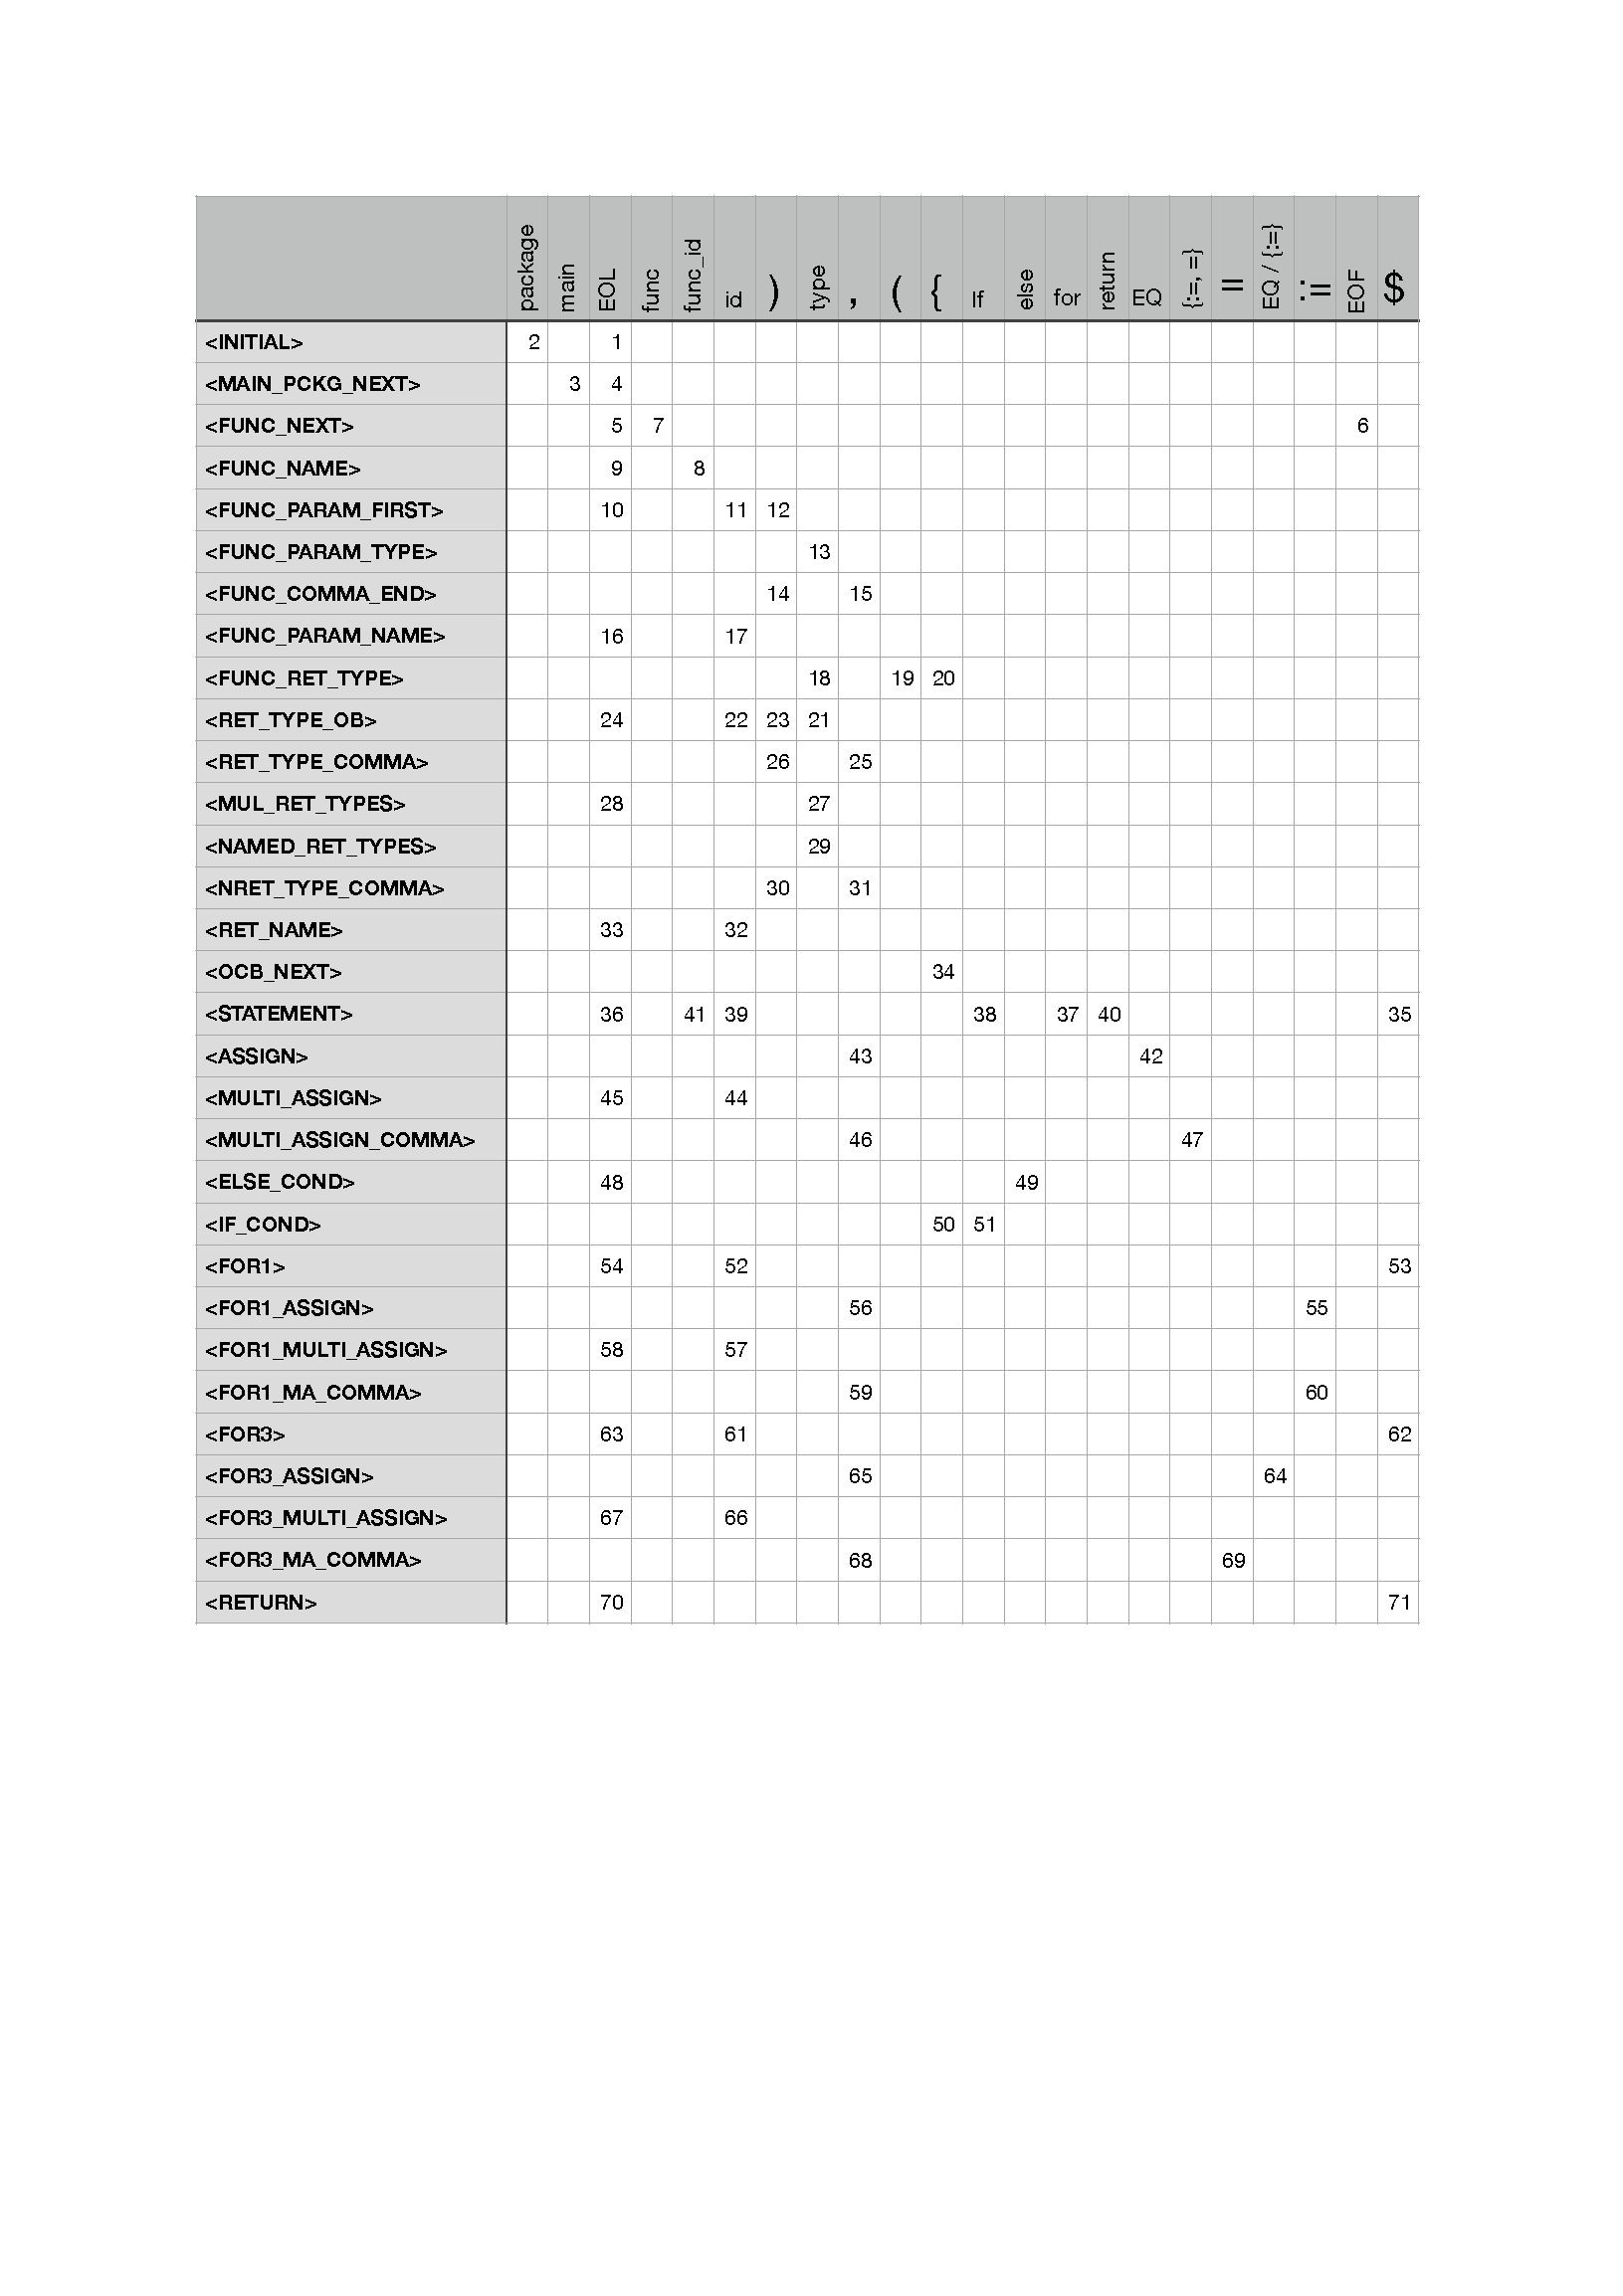
\includegraphics[width=1\linewidth]{img/parsing_table.pdf}
		\caption{Parsing table based on the given LL-grammar.}
		
\end{figure}	



%%%%%%%%%%%%%%%%%%%%%%%%%%%%%%%%%%%%%%%%
%				          PRECEDENCE TABLE 
%%%%%%%%%%%%%%%%%%%%%%%%%%%%%%%%%%%%%%%%
\newpage
\begin{figure}[H]
\section{Precedence Table}
\label{sec:prectable}
\texttt{\bf{L1}} \texttt{= \{+, -, !\}} – unary operators\\
\texttt{\bf{L2}} \texttt{= \{*, /\}}\\
\texttt{\bf{L3}} \texttt{= \{+,  -\}} – binary operators\\
\texttt{\bf{L4}} \texttt{= \{==, !=, >=, <=, >, <\}}\\
\texttt{\bf{L5}} \texttt{= \{\&\&\}}\\
\texttt{\bf{L6}} \texttt{= \{||\}}\\
\texttt{\bf{L7}} \texttt{= \{comma, +=, -=, *=, /=, =, := \}}\\ 
\\
		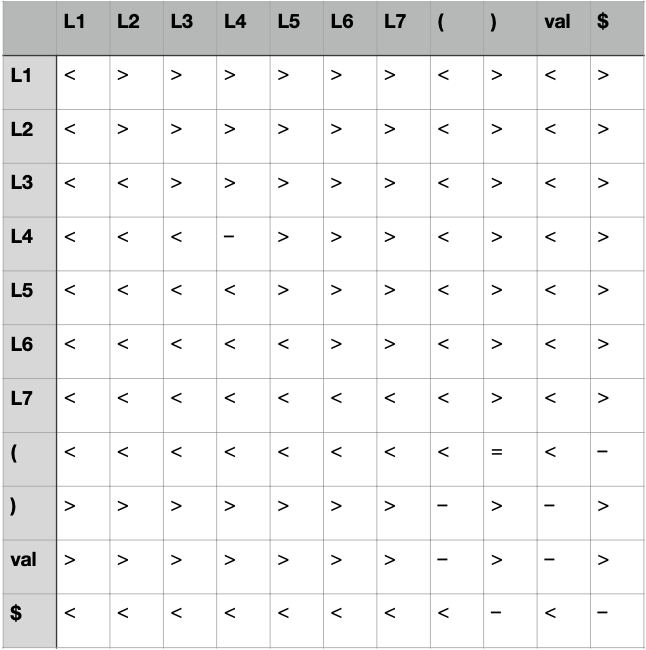
\includegraphics[scale=0.75]{img/table_img.png}
		\caption{Table respresenting the precedence of operators.}
		\label{figure:fsm}
\end{figure}

%%%%%%%%%%%%%%%%%%%%%%%%%%%%%%%%%%%%%%%%
%				    FINITE STATE AUTOMATA
%%%%%%%%%%%%%%%%%%%%%%%%%%%%%%%%%%%%%%%%
\section{Finite State Automata}
\label{figure:fsm}
\begin{figure}[H]
		\centering
		\hspace*{-1cm}
		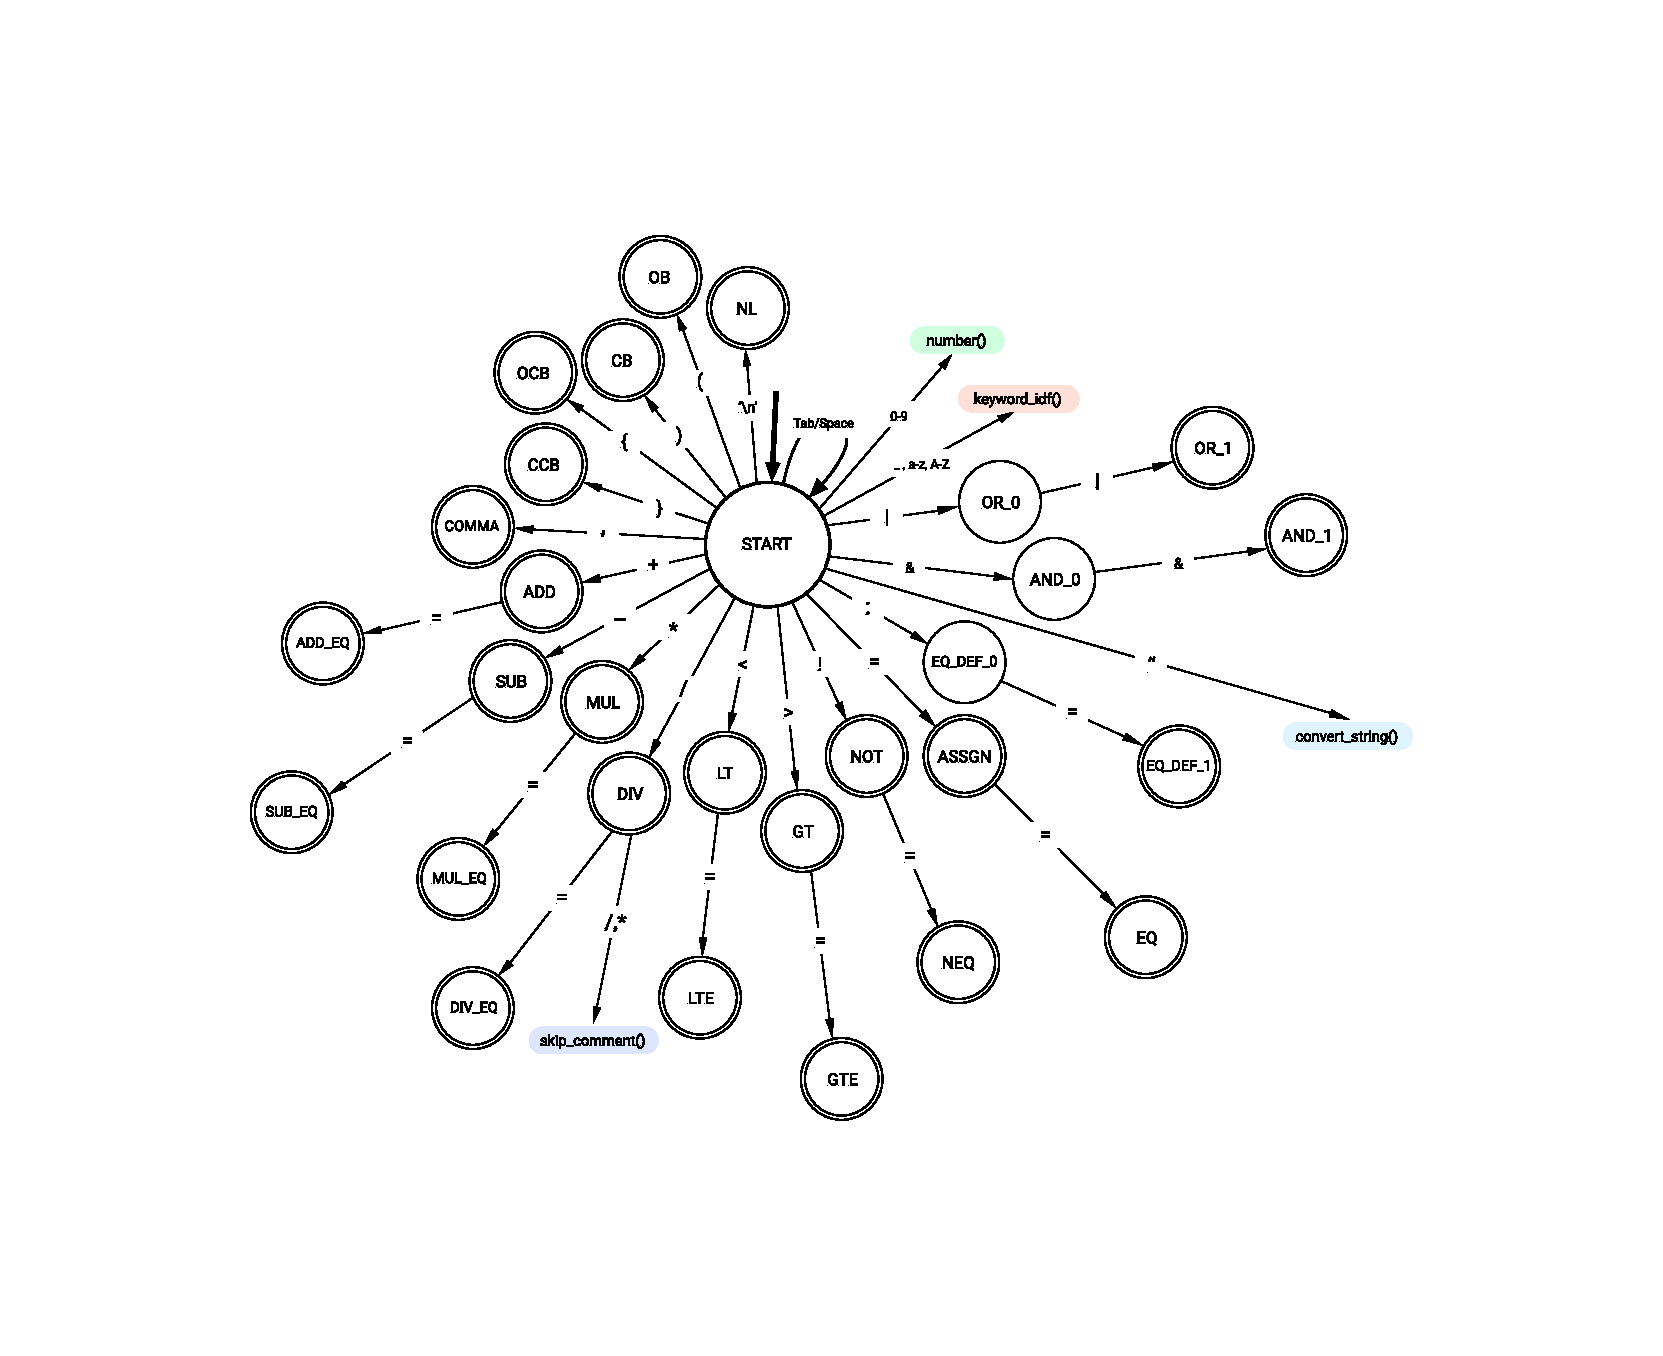
\includegraphics[width=1.2\linewidth]{img/fsm.pdf}
		\hspace*{-1cm}
		\caption{Finite state  automata representing the scanner}
\end{figure}

\begin{figure}[H]
\label{figure:aux_fsm}
		\vspace{-1cm}	
		\centering
		\hspace{-1cm}
		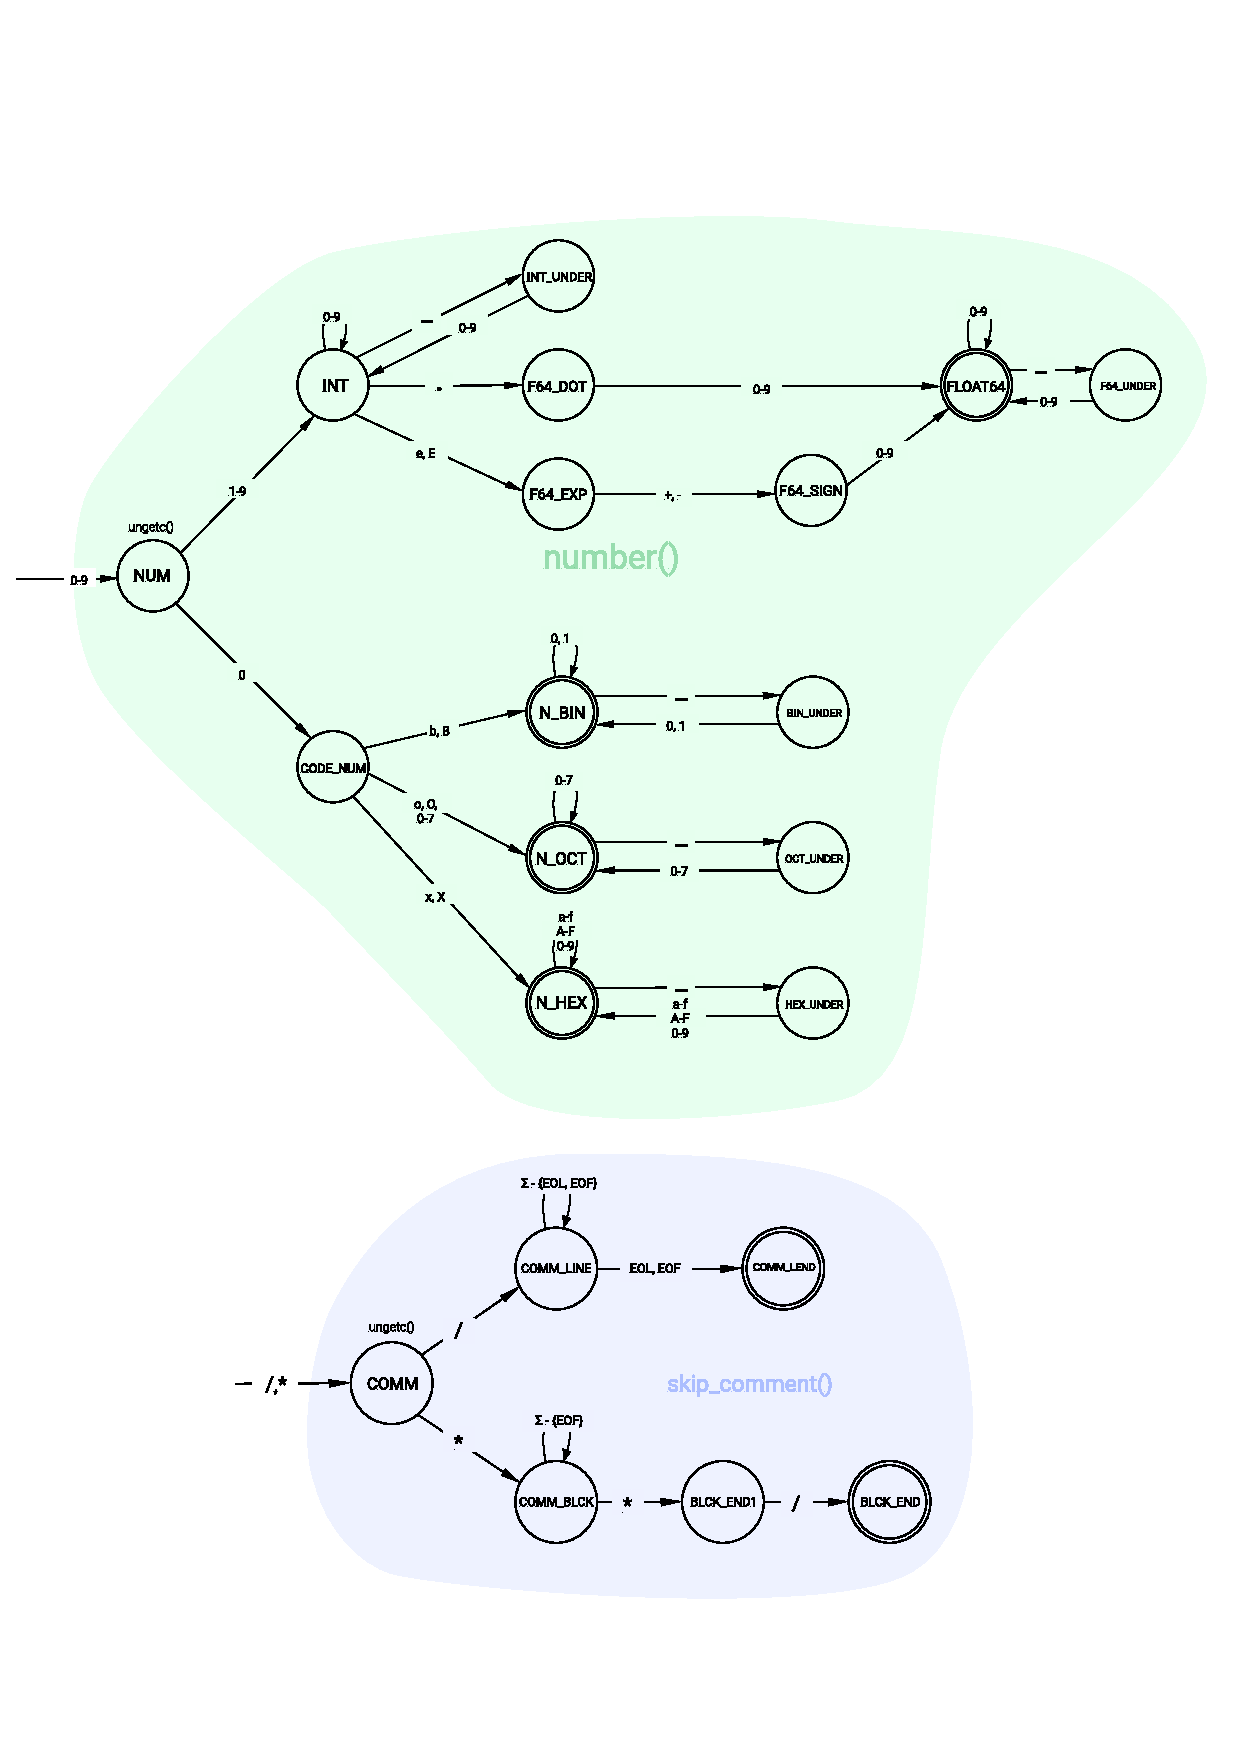
\includegraphics[trim={1cm 1cm -1cm 3.5cm},clip, width=1.15\linewidth]{img/number_fsm.pdf}
		\caption{Auxiliary functions of the scanner}
\end{figure}
\begin{figure}[H]

		%\vspace{-3cm}
		\hspace{-1.2cm}
		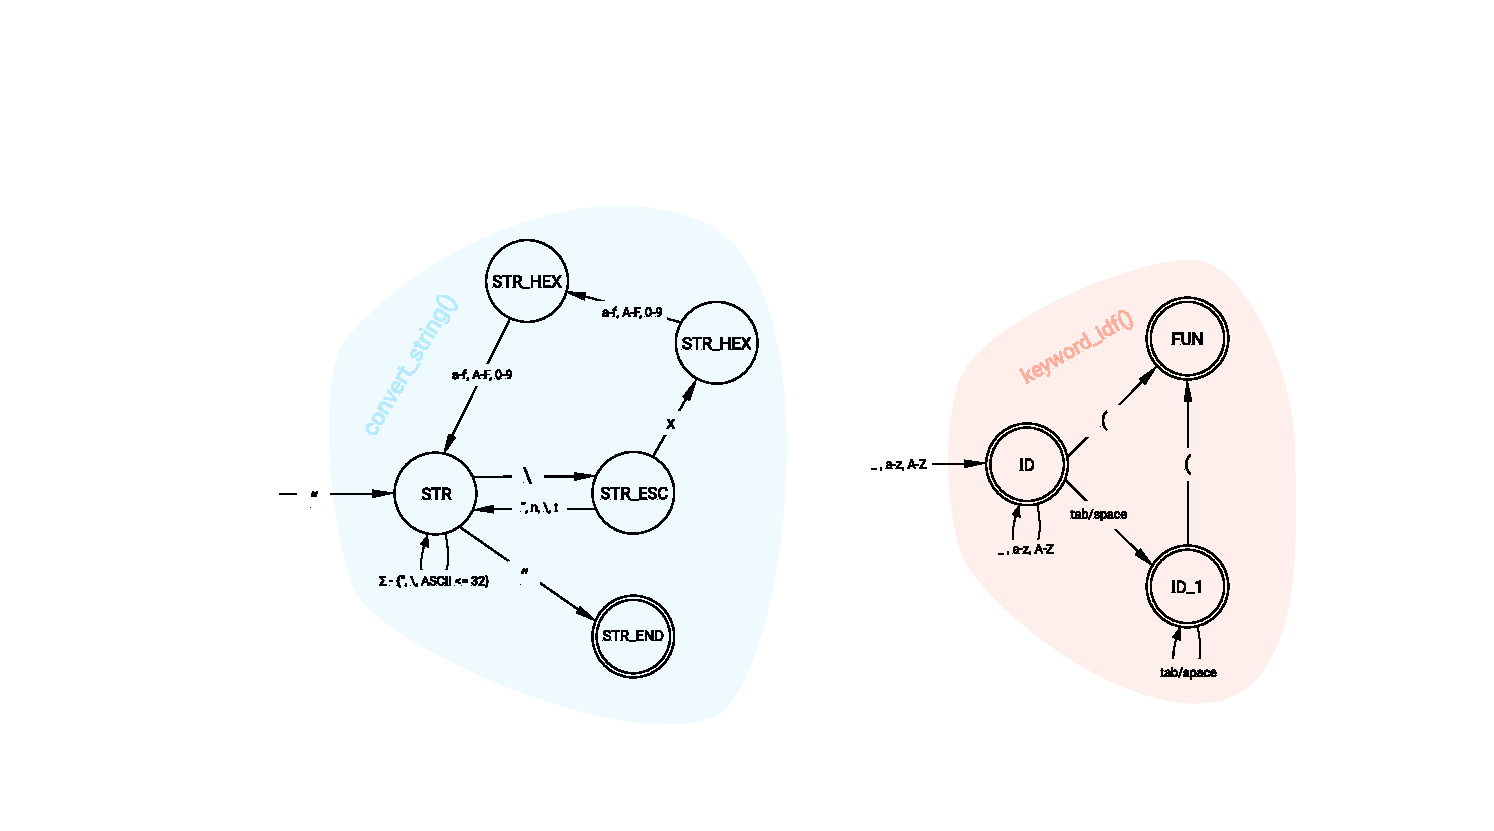
\includegraphics[trim=1cm 1cm 1cm 1cm, clip, width=1.2\linewidth]{img/aux_func.pdf}
		
		\caption{Auxiliary functions of the scanner}
\end{figure}
\vspace{0.5cm}
\hspace{-0.6cm}EOL - end of line\\
EOF - end of file\\
$\Sigma$ - alphabet except of EOF\\
\\
States \texttt{ID} and \texttt{ID\_1} can also \hyperref[sec:retsymbols]{return} a \texttt{keyword} token type, if the read identifier matches with\\a table of keywords or a \texttt{constant} if the read identifier is \texttt{true} or \texttt{false}.





%%%%%%%%%%%%%%%%%%%%%%%%%%%%%%%%%%%%%%%%
%				    AUXILIARY STRUCTURES
%%%%%%%%%%%%%%%%%%%%%%%%%%%%%%%%%%%%%%%%
\begin{figure}
\section{Examples}
\label{sec:examples}
\subsection{Hash Tables Design}
\begin{center}
		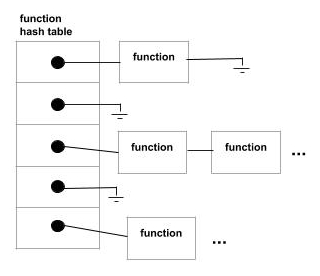
\includegraphics[scale=3.5]{img/FHT.jpg}
		\caption{Hash table of functions}
		\vspace{1.5cm}
		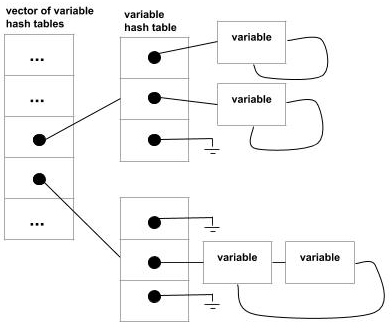
\includegraphics[scale=3.5]{img/VHT.jpg}
		\caption{Hash tables of variables}
\end{center}
\end{figure}
\newpage
\begin{figure}
\subsection{Hash Tables Usage}
\subsubsection{IFJ20 Source Code Example}
\texttt{package main}\\

\texttt{func foo() (int) \{ \textcolor{comment}{// 1. function definition}}

\hspace{0.8cm} \texttt{x := 4 \textcolor{comment}{// 2. variable definition}}

\hspace{0.8cm} \texttt{if x > 3 \{ \textcolor{comment}{// 3. start of a new scope}}

\hspace{1.6cm} \texttt{x := 6 \textcolor{comment}{// 4. variable definition}}

\hspace{0.8cm} \texttt{\} \textcolor{comment}{// 5. end of a scope}}

\hspace{0.8cm}\texttt{return x}

\texttt{\}\\
\\
func main() \{ \textcolor{comment}{// 6. another function definition}\\
\}}\\
\subsubsection{IFJ20 Source Code Explanation}
\begin{enumerate}
\item{Newly added function to the function hash table is assigned with a new variable hash table. The assigned slot in the vector of variable hash tables becomes active.}
\item{Newly defined variable \texttt{x} is stored into the currently active variable hash table on scope level 0.}
\item{Parser scope counter is increased.}
\item{Newly define variable \texttt{x} with the same name, therefore the same hash function, but in higher scope (1). The variable is stored to the variable hash table in front of the variable from lower scope, so it can be found first.}
\item{Rotating with the circular linked list until all variables of currently closed scope are marked as inactive.}
\item{Currently used variable hash table is deactivated, the process continues with action 1.}
\end{enumerate}
\vspace{8cm}
\end{figure}
\newpage
\begin{figure}
\subsubsection{Graphical Example}
		\vspace{1cm}
		\hspace{-2.2cm}
		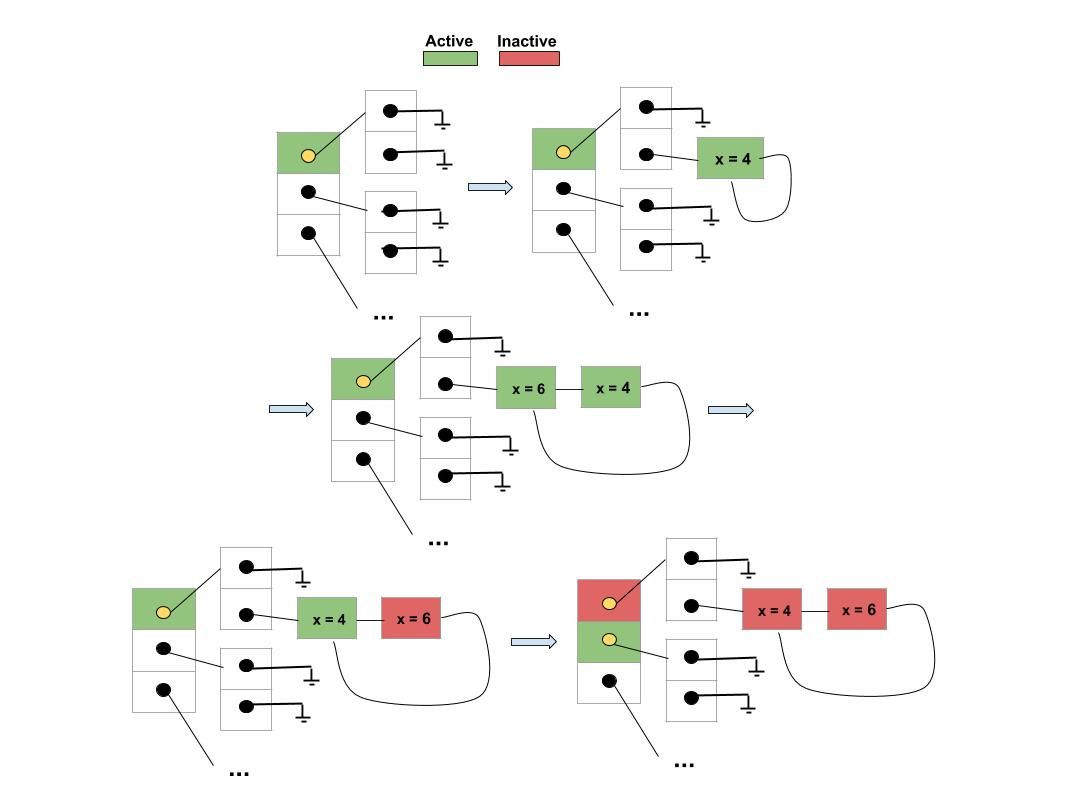
\includegraphics[scale=0.6]{./img/Graphic_ex.jpg}
		\caption{Example of development of the hash table during execution time}
		\vspace{4cm}
\end{figure}
\newpage
\begin{figure}
\subsection{Optimization}
\subsubsection{IFJ20 Source Code Example}
\texttt{package main}\\
\\
\texttt{func foo (x int, y float64) int \{}

\hspace{0.8cm}\texttt{return x+float2int(y)}

\texttt{\}}
\\

\texttt{func main() \{}

\hspace{0.8cm}\texttt{a := 1+2\**6/(5+2-1)\**2}

\hspace{0.8cm}\texttt{b := 3\**a-5}

\hspace{0.8cm}\texttt{c, \_ := inputf()}

\hspace{0.8cm}\texttt{d := int2float(a+b)}
\\

\hspace{0.8cm}\texttt{if a > b \{}

\hspace{1.6cm}\texttt{b = a}

\hspace{0.8cm}\texttt{\} else if c >= d \{}

\hspace{1.6cm}\texttt{print(foo(a\**b, c+d), " ", c, "\textbackslash n")}

\hspace{0.8cm}\texttt{\}}
\\

\hspace{0.8cm}\texttt{b = 5+4\**a\**b/2/a+a}

\hspace{0.8cm}\texttt{print(a, " ", b, "\textbackslash n")}

\texttt{\}}

\subsubsection{Generated IFJcode20 program}
\texttt{.IFJcode20
\\
\textcolor{comment}{\# definition of compiler variables}\\
DEFVAR GF@?temp\&1\\
DEFVAR GF@?temp\&2\\
DEFVAR GF@?temp\&3\\
DEFVAR GF@?temp\&4\\
DEFVAR GF@?temp\&5\\
DEFVAR GF@?temp\&6\\
DEFVAR GF@?\_\&\\
\\
\textcolor{comment}{\# definition of variables of non recursive functions}\\
DEFVAR GF@x\&13\\
DEFVAR GF@y\&14\\
DEFVAR GF@a\&15\\
DEFVAR GF@b\&16\\
DEFVAR GF@c\&17\\
DEFVAR GF@d\&18\\
\\}
\end{figure}
\begin{figure}
\texttt{\textcolor{comment}{\# definition of registers}\\
DEFVAR GF@r\%1\&\\
DEFVAR GF@r\%2\&\\
JUMP \$main\\
\\
\textcolor{comment}{\# \$foo function definition}\\
LABEL \$foo\\
\textcolor{comment}{\# memory frame creation omitted}\\
\textcolor{comment}{\# return x + float2int(y)}\\
PUSHS GF@x\&13\\
\textcolor{comment}{\# float2int() function inlined, with the use of temporarily variable}\\
FLOAT2INT GF@?temp\&1 GF@y\&14\\
PUSHS GF@?temp\&1\\
ADDS\\
\textcolor{comment}{\# value returned on the stack}\\
RETURN\\
\textcolor{comment}{\# definition end}\\
\\
\textcolor{comment}{\# main function definition}\\
LABEL \$main\\
\textcolor{comment}{\# memory frame creation omitted}\\
\\
\textcolor{comment}{\# c, \_ := inputf()}\\
\textcolor{comment}{\# inputf() function inlined}\\
\textcolor{comment}{\# read value is not verified, as the error signifying variable is \_}\\
READ GF@c\&17 float\\
\\
\textcolor{comment}{\# d := int2float(a+b), a == 5, b == 10}\\
\textcolor{comment}{\# direct conversion, with the use of constant propagation}\\
INT2FLOAT GF@d\&18 int@15\\
\\
\textcolor{comment}{\# a := 1+2\**6/(5+2-1)\**2, previously evaluated to a := 5}\\
\textcolor{comment}{\# b := 3\**a-5, previously evaluated to b := 10}\\
\textcolor{comment}{\# preemptive assign of variables with constant value before if statement}\\
MOVE GF@a\&15 int@5\\
MOVE GF@b\&16 int@10\\
\\
\textcolor{comment}{\# if a > b \{}\\
\textcolor{comment}{\# unconditioned jump based on a compile time calculated values}\\
JUMP \$main\_if1\_1\\
\\
\textcolor{comment}{\# b = a}\\
\textcolor{comment}{\# a == 5}\\
MOVE GF@b\&16 int@5\\}
\end{figure}
\newpage
\begin{figure}
\texttt{\textcolor{comment}{\# \}}\\
JUMP \$main\_ifend1\\
LABEL \$main\_if1\_1\\
\\
\textcolor{comment}{\# else if c >= d \{}\\
\textcolor{comment}{\# calculation of GTE by using LT and NOT}\\
\textcolor{comment}{\# use of a register for storing intermediate result}\\
LT GF@r\%1\& GF@c\&17 GF@d\&18\\
JUMPIFNEQ \$main\_if1\_2 GF@r\%1\& bool@false\\
\\
\textcolor{comment}{\# foo(a\**b, c+d), a == 5, b == 10}\\
\textcolor{comment}{\# assigning/calculating the parameters of called function}\\
MOVE GF@x\&13 int@50\\
ADD GF@y\&14 GF@c\&17 GF@d\&18\\
CALL \$foo\\
\textcolor{comment}{\# assigning the return value from the stack after a function call}\\
POPS GF@?temp\&1\\
\\
\textcolor{comment}{\# print(foo(a\**b, c+d), " ", c, "\textbackslash n")}\\
\textcolor{comment}{\# print() function inlined}\\
WRITE GF@?temp\&1\\
WRITE string@\textbackslash 032\\
WRITE GF@c\&17\\
WRITE string@\textbackslash 010\\
\\
\textcolor{comment}{\# \}}\\
LABEL \$main\_if1\_2\\
LABEL \$main\_ifend1\\
\\
\textcolor{comment}{\# b = 5+4\**a\**b/2/a+a}\\
\textcolor{comment}{\# the value of variable b is unknown after the if statement, a == 5}\\
\textcolor{comment}{\# 4\**a is reduced to 20}\\
MUL GF@r\%2\& int@20 GF@b\&16\\
\textcolor{comment}{\# 2/a is reduced to 10 (operator inversion)}\\
IDIV GF@r\%2\& GF@r\%2\& int@10\\
\textcolor{comment}{\# 5+...+a - separated constants reduced to 10}\\
ADD GF@b\&16 int@10 GF@r\%2\&\\
\\
\textcolor{comment}{\# print(a, " ", b, "\textbackslash n"), a == 5}\\
\textcolor{comment}{\# print() function inlined}\\
WRITE int@5\\
WRITE string@\textbackslash 032\\
WRITE GF@b\&16\\
WRITE string@\textbackslash 010\\
\\
EXIT int@0\\
\textcolor{comment}{\# definition end\\}}
\vspace{20cm}
\end{figure}
	
\end{document}
